\section*{Постановка задачи}

\textbf{Задание:} используя хвостовую рекурсию, разработать эффективную программу (комментируя назначение аргументов), позволяющую:
\begin{enumerate}
	\item Найти длину списка (по верхнему уровню);
	\item Найти сумму элементов числового списка;
	\item Найти сумму элементов числового списка, стоящих на нечетных позициях исходного списка (нумерация от 0);
\end{enumerate}

\begin{lstinputlisting}[label=third,caption=Решение задания №1, language=prolog, firstline=1, lastline=47]{../src/lab_17.pro}
\end{lstinputlisting}

\begin{figure}[H]
	\caption{Таблица к заданию.}
	\begin{center}
		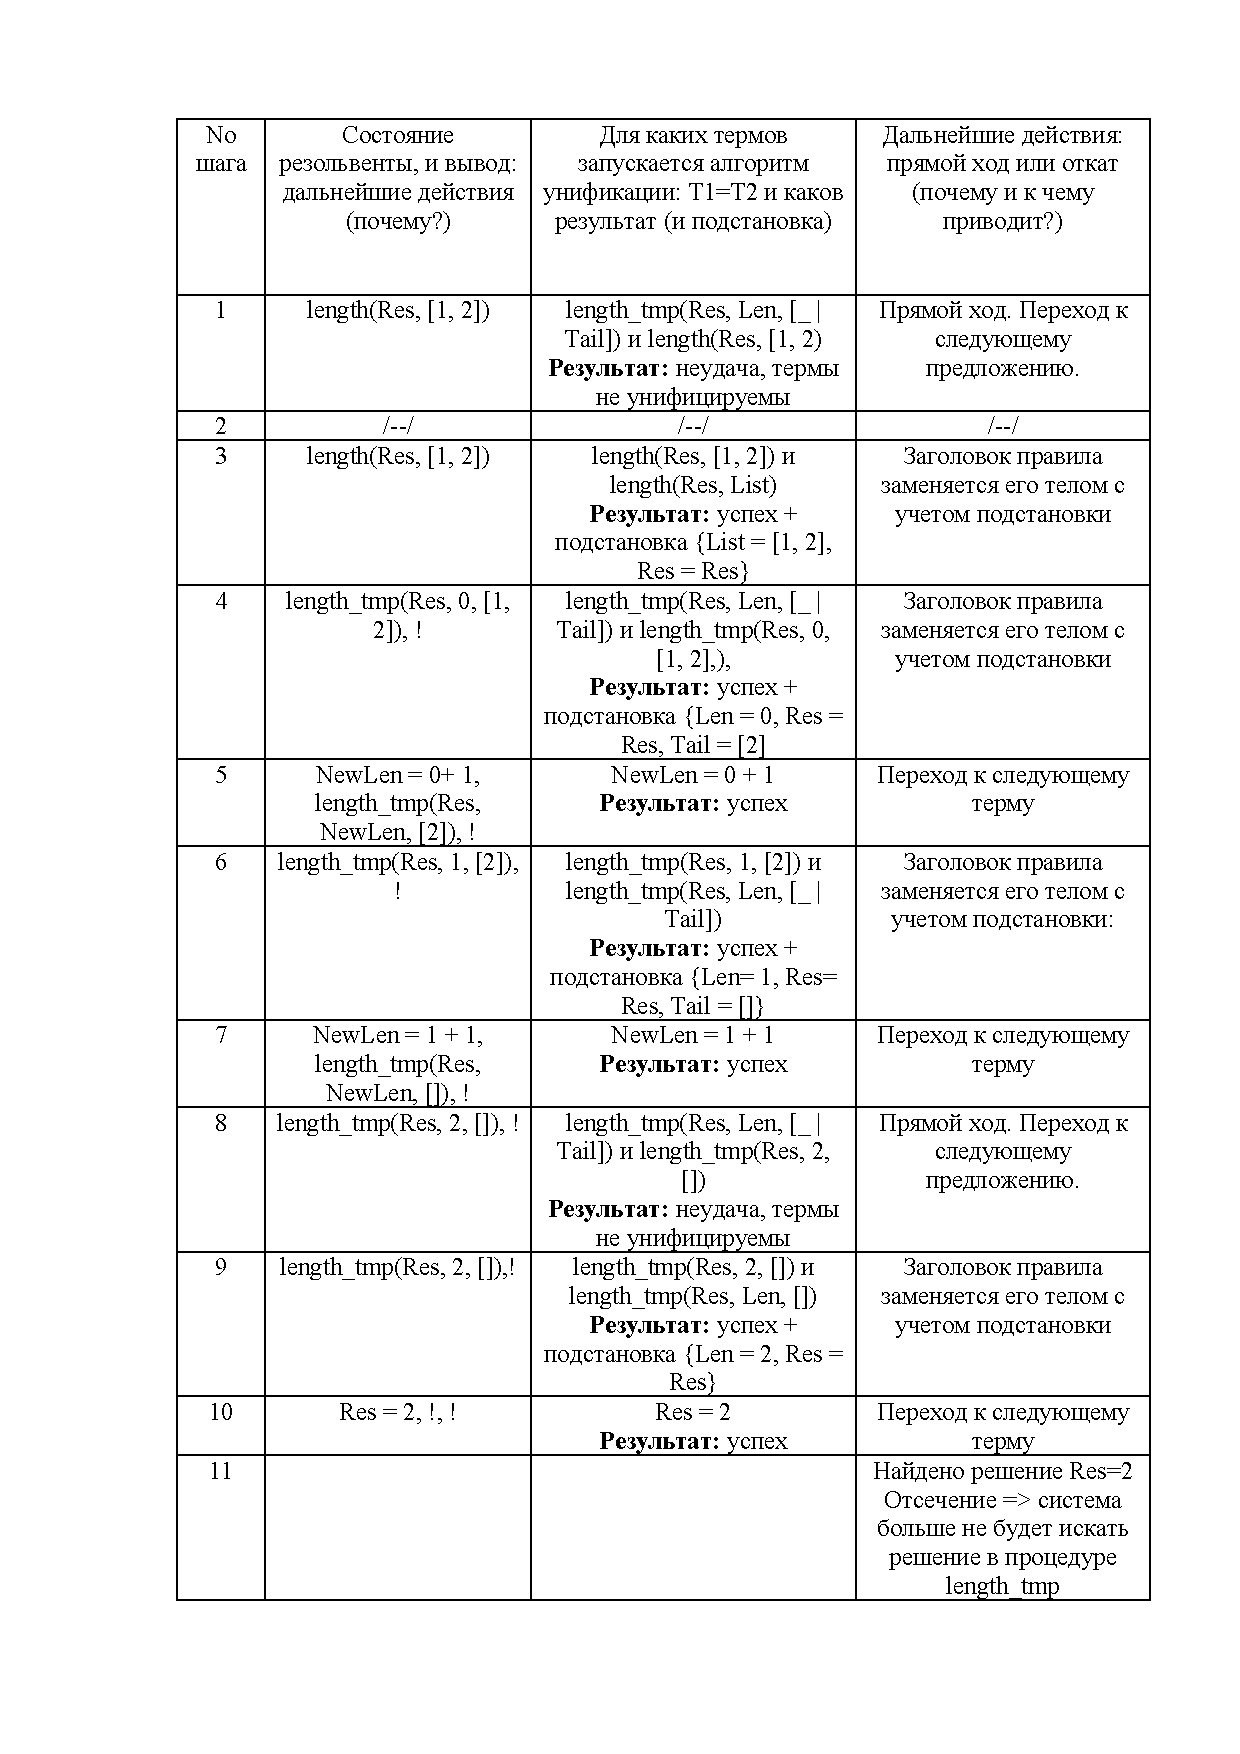
\includegraphics[scale=0.85]{img/16.1.pdf}
	\end{center}
	
\end{figure}
